
%(BEGIN_QUESTION)
% Copyright 2011, Tony R. Kuphaldt, released under the Creative Commons Attribution License (v 1.0)
% This means you may do almost anything with this work of mine, so long as you give me proper credit

This liquid storage tank happens to have three precision pressure transmitters mounted at different heights.  The lowest transmitter is at ground level, while the next one is exactly 6 feet above ground level and the third is at the very top of the vessel (25 feet up from the bottom):

$$\includegraphics[width=15.5cm]{i03454x01.eps}$$

Calculate the level of liquid inside the vessel as well as its density in units of pounds per cubic foot:

\vskip 10pt

Level = \underbar{\hskip 50pt} feet (from ground level)

\vskip 10pt

Liquid density = \underbar{\hskip 50pt} pounds per cubic foot 

\underbar{file i03454}
%(END_QUESTION)





%(BEGIN_ANSWER)

Level = \underbar{\bf 12.38 feet} ; Density = \underbar{\bf 53.04} lb/ft$^{3}$

\vskip 10pt

5 points for correct level, 5 points for correct density.

%(END_ANSWER)





%(BEGIN_NOTES)

{\bf This question is intended for exams only and not worksheets!}.

%(END_NOTES)

